\section{Wave steering and micro-inertia}
\label{sec:steering}

The band results show that orientation redistributes the spectrum; the corresponding energy-flow direction is assessed here from the group velocity. The section then relates this steering response to gradient-energy participation and the high-wavenumber transverse-wave limit.

\subsection{Group-velocity steering}
On the constant-wavenumber ring $|\bmk|=\bar{k}=0.5$, anisotropy makes the group velocity non-collinear with the wave vector. Figure~\ref{fig:ifc_wave_steering} shows the angular deviation $\delta(\phi)=\angle\bmv_g-\angle\bmk$ and the group-velocity magnitude for $\theta=45^\circ$. The peak deviation increases from $0^\circ$ at $\mathrm{AR}=1$ to $1.4146^\circ$ at $\mathrm{AR}=5$ and $2.7846^\circ$ at $\mathrm{AR}=10$, indicating progressively stronger directional variation in energy transport. The accompanying modulation in $|\bmv_g|$ shows that orientation also changes the energy-transport speed around the contour.

\begin{figure}[htbp]
\centering
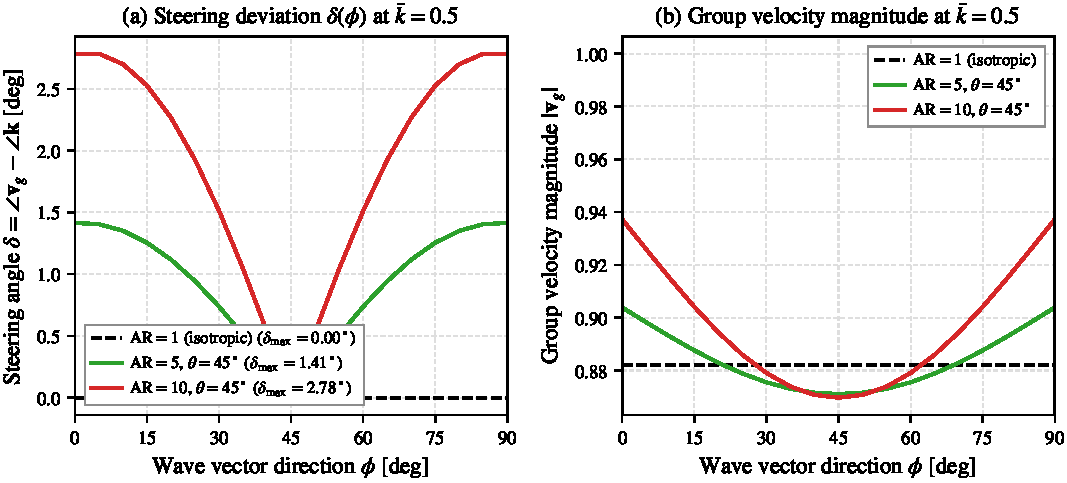
\includegraphics[width=\textwidth]{figures/fig12_ifc_wave_steering.pdf}
\caption{Acoustic-branch group-velocity steering on $|\bmk|=0.5$ at $\theta=45^\circ$. (a) Angular deviation for $\mathrm{AR}=1,5,10$, with peak values $0^\circ$, $1.4146^\circ$, and $2.7846^\circ$. (b) Directional variation of group-velocity magnitude.}
\label{fig:ifc_wave_steering}
\end{figure}

\subsection{Orientation repositions the steering lobes}
The orientation sweep in Figure~\ref{fig:s7_steering_sweep} and Table~\ref{tab:steering_sweep} evaluates $\theta\in\{0^\circ,15^\circ,\ldots,90^\circ\}$ for $\mathrm{AR}=5$ and $10$ on the same ring and acoustic branch. The peak deviation remains $1.4146^\circ$ and $2.7846^\circ$, respectively, across the sampled orientations to within $10^{-5}\,$deg. The principal direction follows $\phi^*(\theta)\simeq(45^\circ-\theta)\bmod90^\circ$, with excursions of at most $5^\circ$ at $\mathrm{AR}=10$. Thus, over the sampled grid, orientation shifts the steering lobes without materially changing their maximum amplitude.

\begin{figure}[htbp]
\centering
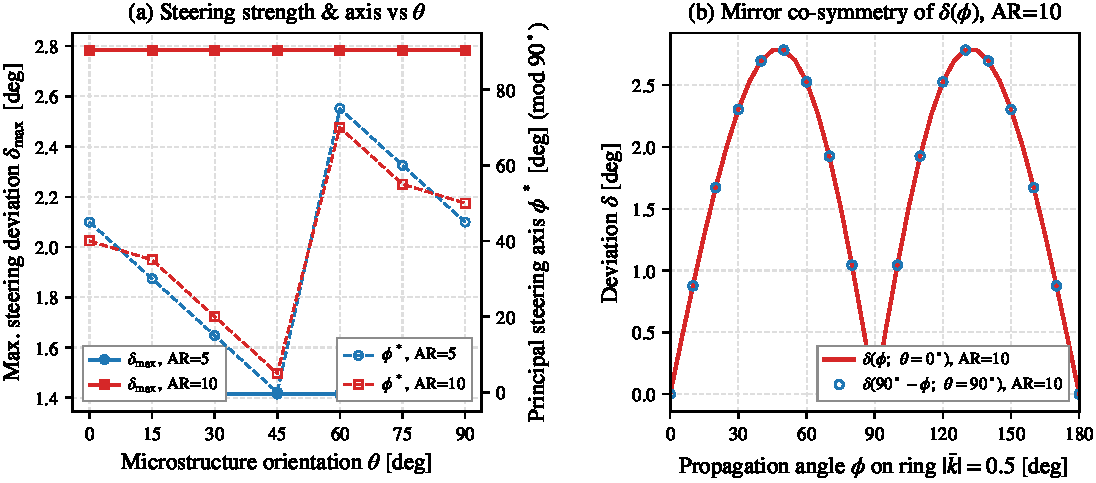
\includegraphics[width=\textwidth]{figures/fig14_s7_steering_sweep.pdf}
\caption{Orientation dependence of steering on $|\bmk|=0.5$. (a) Peak deviation $\delta_{\max}$ and principal direction $\phi^*$ for $\mathrm{AR}=5,10$; the peak amplitude is invariant over the sampled orientations, while the lobe direction follows the rotated tensor axes on the $5^\circ$ ring grid. (b) The $\theta=0^\circ$ and $90^\circ$ deviation fields at $\mathrm{AR}=10$ exhibit mirror co-symmetry.}
\label{fig:s7_steering_sweep}
\end{figure}

\begin{table}[htbp]
\centering
\caption{Peak group-velocity deviation and principal steering direction across the sampled orientations at $\bar{k}=0.5$.}
\label{tab:steering_sweep}
% Auto-generated by tab07_steering_sweep.py from p12b_s7_theta_sweep_mesh16.json - DO NOT EDIT MANUALLY
\begin{tabularx}{\textwidth}{@{}c r r r r@{}}
\toprule
$\theta$ & \multicolumn{2}{c}{$\mathrm{AR}=5$} & \multicolumn{2}{c}{$\mathrm{AR}=10$} \\
\cmidrule(lr){2-3}\cmidrule(lr){4-5}
 & $\delta_{\max}$ [deg] & $\phi^*$ [deg] & $\delta_{\max}$ [deg] & $\phi^*$ [deg] \\
\midrule
$0^\circ$ & 1.4146 & 45 & 2.7846 & 40 \\
$15^\circ$ & 1.4146 & 30 & 2.7846 & 35 \\
$30^\circ$ & 1.4146 & 15 & 2.7846 & 20 \\
$45^\circ$ & 1.4146 & 0 & 2.7846 & 5 \\
$60^\circ$ & 1.4146 & 75 & 2.7846 & 70 \\
$75^\circ$ & 1.4146 & 60 & 2.7846 & 55 \\
$90^\circ$ & 1.4146 & 45 & 2.7846 & 50 \\
\midrule
\multicolumn{5}{@{}>{\raggedright\arraybackslash}p{\dimexpr\textwidth-2\tabcolsep\relax}@{}}{$M_s = \phi^*(90^\circ) - \phi^*(0^\circ)$: $M_s(\mathrm{AR}{=}5) = +0.0000^\circ$, $M_s(\mathrm{AR}{=}10) = +10.0000^\circ$ (locked $5^\circ$ grid; parabolic refinement of the peak lies within one sampling step of these figures, so the sweep does not resolve any finer value)}\\
\multicolumn{5}{@{}>{\raggedright\arraybackslash}p{\dimexpr\textwidth-2\tabcolsep\relax}@{}}{Symmetries verified numerically ($\le 1.3\times 10^{-6}\,$deg for both headless and mirror): $\delta(\phi;\theta)=\delta(\phi+180^\circ;\theta)$ (headless) and $\delta(\phi;\theta)=\delta(90^\circ-\phi;\,90^\circ-\theta)$ (mirror).}\\
\bottomrule
\end{tabularx}

\end{table}

Defining the sampled steering measure as
\begin{equation}
M_s(\mathrm{AR})=\phi^*(90^\circ,\mathrm{AR})-\phi^*(0^\circ,\mathrm{AR}),
\label{eq:Ms_def}
\end{equation}
the values are
\begin{equation}
M_s(\mathrm{AR}=5)=0^\circ,\qquad M_s(\mathrm{AR}=10)=10^\circ.
\label{eq:Ms_value}
\end{equation}
The $5^\circ$ ring-sampling step limits the resolution of this difference. The deviation field also satisfies headless periodicity and mirror co-symmetry to residuals no greater than $1.3\times10^{-6}\,$deg; the peak amplitude is invariant under $\theta\mapsto90^\circ-\theta$ to within $10^{-7}\,$deg. These symmetries explain why orientation principally repositions the lobes rather than increasing the sampled peak deviation.

\subsection{Gradient energy and the high-wavenumber limit}
For Mindlin Form-II elasticity, the strain energy is the sum of the classical and gradient contributions, $W=W_c+W_g$, with $W_c=\tfrac12\int_\Omega\sigma_{ij}\varepsilon_{ij}\,\dif\Omega$ and $W_g=\tfrac12\int_\Omega\tau_{ijk}\eta_{ijk}\,\dif\Omega$. Along $\Gamma$--$X$, the gradient-energy fraction rises from $0.20\%$ at $\bar{k}=0.1$ to $16.49\%$ at $\bar{k}=1.0$ (Figure~\ref{fig:energy_microinertia}), showing the increasing contribution of double-stress work as the wavelength approaches the cell scale.

\begin{figure}[htbp]
\centering
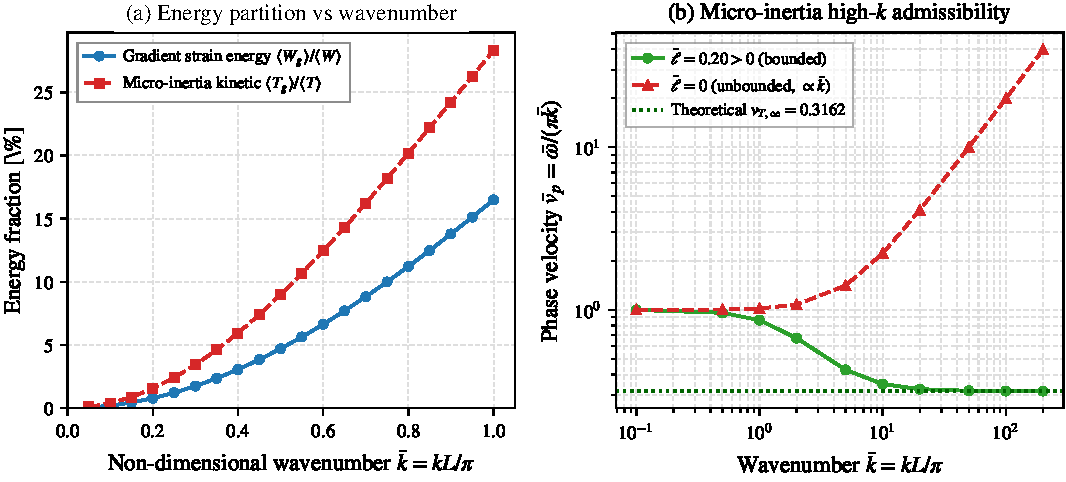
\includegraphics[width=\textwidth]{figures/fig13_energy_microinertia.pdf}
\caption{(a) Gradient-energy fraction $W_g/W$ versus wavenumber. (b) Transverse-branch phase velocity with and without gradient micro-inertia; the finite high-wavenumber limit is specific to the shear branch analyzed here.}
\label{fig:energy_microinertia}
\end{figure}

For the transverse shear branch considered in Appendix~\ref{app:asymptotics}, the model predicts
\begin{equation}
\bar{v}_{T,\infty}=\frac{\bar{l}_{\mathrm{eff}}}{\sqrt{10}\,\bar{\ell}_{\mathrm{i}}}=\frac{0.20}{\sqrt{10}\times0.20}=\frac{1}{\sqrt{10}}\approx0.3162.
\label{eq:v_horizon_sec7}
\end{equation}
At $\bar{k}=200$, the computed phase speed with micro-inertia is $0.3163$, within $0.03\%$ of this asymptote. In the corresponding no-micro-inertia model, the analytical branch relation grows without bound; the computed phase speed reaches $39.75$ at $\bar{k}=200$. This comparison concerns the stated transverse-branch model and does not establish a general speed bound for other branches or constitutive settings.
